\documentclass[aip, jcp, reprint, onecolumn, nofootinbib]{revtex4-2}

\bibliographystyle{apsrev4-2}

\usepackage{physics}
\usepackage{amsmath}
\usepackage{amssymb}
\usepackage{mathtools}
\usepackage{graphicx}
\usepackage{dcolumn}
\usepackage[colorlinks=true, linkcolor=black, urlcolor=blue, citecolor=black, anchorcolor=black]{hyperref}

%supplementary figs
\renewcommand{\thefigure}{S\arabic{figure}}
\renewcommand{\thetable}{S\arabic{table}}
\renewcommand\theequation{S\arabic{equation}}
\renewcommand*{\thepage}{S\arabic{page}}

\graphicspath{{"figures/"}}
\begin{document}
%Title of paper
\title{Supplementary Material: Coherent IR-Hyper-Raman Four Wave Mixing Spectroscopy}


\author{Ryan P. McDonnell} 
\author{Daniel D. Kohler}
\author{John C. Wright} \email{wright@chem.wisc.edu}

\affiliation{Department of Chemistry, 
        University of Wisconsin - Madison, 
        Madison, Wisconsin 53706, 
        United States of America}

%\date{\today}

\maketitle
\tableofcontents
\clearpage


\section{Evaluating Herzberg-Teller Integrals for Harmonic Wells of Identical Curvature}

In this section, we discuss the evaluation of Herzberg-Teller integrals when the ground and first excited state are harmonic wells of identical curvature.\cite{HerzbergTeller1933}
We investigate the one dimensional case using the Hamiltonian described in the main text, $H = H_g |g) \left(g| + H_e |e\right) (e|$, where
\begin{subequations}\label{Hamiltonian}
	\begin{equation}
		H_g = \frac{\hbar \omega }{2} \left(p^2 + q^2 \right)
	\end{equation}
	and
	\begin{equation}
		H_e = \frac{\hbar \omega }{2} \left(p^2 +  (q-\Delta)^2 \right) + \hbar \omega_{eg}.
	\end{equation} 
\end{subequations}
Here, $p,q$ are the dimensionless conjugate normal mode coordinates, $\hbar\omega_{eg}$ is the energy difference between $|e)$ and $|g)$, and $\Delta$ is the dimensionless offset of the excited state surface relative to the ground state.
The Hamiltonians $H_g$ and $H_e$ are quantum harmonic oscillators.
The harmonic oscillator wavefunctions are well known, and their position space forms are
\begin{equation}
	\psi_m(q) = \langle q | m \rangle = N_m H_m(q) \exp(-\frac{q^2}{2}),
\end{equation}
where $N_m = (m! \ 2^m \pi^{\frac{1}{2}})^{-\frac{1}{2}}$ is the normalization factor and $H_m$ is the $m^\text{th}$ Hermite Polynomial.\cite{RN230, MorseFeshbach}

For an $n$-quantum excited state vibration $| \tilde{n} \rangle$ and a $m$-quantum ground state vibration $\ket{m}$, the $k^\text{th}$ order vibrational coupling term is
\begin{equation}
	\begin{split}
		\mel{\tilde{n}}{q^k}{m} &= \int_{-\infty}^\infty \mathrm{d}q \ \psi^*_n(q-\Delta) q^k \psi_m(q)\\
		&= \int_{-\infty}^\infty \mathrm{d}q \ N_n H_n(q-\Delta) \exp(-\frac{(q - \Delta)^2}{2}) q^k N_m H_m(q) \exp(-\frac{q^2}{2}) \\
		&= N_n N_m \exp(-\frac{\Delta^2}{2}) \int_{-\infty}^\infty \mathrm{d}q \ H_n(q-\Delta) q^k H_m(q) \exp(-q^2 + q\Delta).
	\end{split}\label{key}
\end{equation}
The integral corresponds to Franck-Condon factors for $k=0$ and Herzberg-Teller integrals for $k=1$.
The vibrational coupling integrals are written assuming the dipole moment is Taylor expanded about the equilibrium point of the ground state geometry ($q=0$), as done in the main text.
Note that in the limit $\Delta \rightarrow 0$, typical harmonic oscillator selection rules are restored as the two wells have the same vibrational Hamiltonian and thus share a subspace of orthonormal eigenstates.

\subsection{General Solution to $\langle \tilde{n} | q^k | m \rangle$}
The matrix elements of \autoref{key} can be computed numerically, but analytic forms of the integral also exist. 
Due to the polynomial nature of $H_v(q)$, the product $H_n(q-\Delta) q^k H_m(q)$ will also be a polynomial, so that the integral in \autoref{key} will be of the form
\begin{eqnarray}\label{eq:Pnmkdef}
	\int_{-\infty}^\infty \mathrm{d}q \ P_{nmk}(q) \exp(-q^2 + q\Delta), \\
	P_{nmk}(q) \equiv \sum_\lambda^{n+m+k} a_\lambda q^\lambda
\end{eqnarray}
for some set coefficients $a_\lambda$ to be specified later. 
As a result, we can recast \autoref{key} into the linear combination of integrals
\begin{equation}\label{eq:analytic_form}
	\mel{\tilde{n}}{q^k}{m} = N_n N_m \exp(-\frac{\Delta^2}{2}) \sum_\lambda a_\lambda F_\lambda(\Delta),
\end{equation}
where
\begin{equation}\label{integral}
	F_w(\Delta) \equiv \int_{-\infty}^\infty \mathrm{d}q \ q^w \exp(-q^2 + q\Delta).
\end{equation}
\autoref{integral} can be readily evaluated, as we now show. 
 When $w=0$, the integral is evaluated by completing the square:\footnote{$\int_{-\infty}^{\infty} \mathrm{d}x \exp(-(x-a)^2) = \sqrt{\pi}$}
\begin{equation}
	\begin{split}
		F_0(\Delta) & =  \int_{-\infty}^\infty \mathrm{d}q \exp\left(-q^2 + q\Delta\right)\\
		&= \int_{-\infty}^\infty \mathrm{d}q \exp(-(q^2 - q\Delta +\frac{\Delta^2}{4} - \frac{\Delta^2}{4}))\\
		&= \exp(\frac{\Delta^2}{4}) \int_{-\infty}^\infty \mathrm{d}q \exp(-(q - \frac{\Delta}{2})^2) \\
		&= \sqrt{\pi} \exp(\frac{\Delta^2}{4}).
	\end{split}
\end{equation}
For the general solution, \autoref{integral} is evaluated via repeated use of a well-known Gaussian identity
\begin{equation}\label{identity}
	\begin{split}
		F_w(\Delta) &= \int_{-\infty}^\infty \mathrm{d}q \ q^w \exp(-q^2 + q\Delta) = \partial_{\Delta} \int_{-\infty}^\infty \mathrm{d}q \ q^{w-1} \exp(-q^2 + q\Delta) \\
		&= \frac{\mathrm{d}}{\mathrm{d}\Delta} F_{w-1}(\Delta)
	\end{split}
\end{equation}
so we can write\footnote{
	Rearranging the Hermite polynomial generator so that $\frac{\mathrm{d}^n}{\mathrm{d}x^n} e^{-x^2} = (-1)^n H_n(x) e^{-x^2}$, setting $x \ = \ i \Delta /2$ and using the chain rule ($\frac{\mathrm{d}}{\mathrm{d}x} =  \frac{\mathrm{d}}{\mathrm{d}\Delta}  \frac{\mathrm{d\Delta}}{\mathrm{d}x}$) provides the final result in \autoref{eq:F_solved}.
	}
\begin{equation}\label{eq:F_solved}
	\begin{split}
		F_w(\Delta) &= \frac{\mathrm{d}^w}{\mathrm{d}\Delta^w} F_0(\Delta) \\
		&= \sqrt{\pi} \frac{\mathrm{d}^w}{\mathrm{d}\Delta^w} \exp(\frac{\Delta^2}{4}) \\
		&= \sqrt{\pi} \left( -\frac{i}{2} \right)^w \exp(\frac{\Delta^2}{4}) H_w\left(i\frac{\Delta}{2}\right).
	\end{split}
\end{equation}
In the last line we have used the generator definition of Hermite polynomials:  $H_n(x) \equiv (-1)^n e^{x^2} \frac{\mathrm{d}^n}{\mathrm{d}x^n} e^{-x^2}$.\cite{MorseFeshbach}
\vspace{3pt}

We now will evaluate the polynomial coefficients $P_{nmk}(q)$.
The Hermite polynomials of \autoref{key} can be explicitly written as\cite{MorseFeshbach}
\begin{equation}
\begin{split}
	H_m(q) &= \sum_{s=0}^{\left\lfloor{m/2}\right\rfloor} a_m^{(m-2s)} q^{m-2s}, \\
	H_n(q-\Delta) &= \sum_{s=0}^{\left\lfloor{n/2}\right\rfloor}
	a_n^{(n-2s)} (q-\Delta)^{n-2s} \\
		&= \sum_{s=0}^{\left\lfloor{n/2}\right\rfloor} a_n^{(n-2s)} \sum_{l=0}^{n-2s} \left(-\Delta\right)^{n-2s-l} \binom{n-2s}{l} q^l,
\end{split}
\end{equation}
where $\left\lfloor n \right\rfloor$ denotes the \textit{floor} of $n$, $\binom{a}{b} = a! / (b!(a-b)!)$,\footnote{
	The binomial expansion, $(x-y)^m = \sum_{a=0}^m \binom{m}{a} x^a (-y)^{m-a}$, was used to rewrite $(q-\Delta)^{n-2s}$.
} and the Hermite coefficients are
\begin{equation}
	a_n^{(n-2s)} = n! \frac{(-1)^x 2^{n-2s}}{s!(n-2s)!}.
\end{equation}
Multiplying these terms together give us explicit polynomial coefficients:
\begin{equation}\label{eq:poly_solved}
\begin{split}
	P_{nmk}(q) %&= \sum_{x=0}^{\left\lfloor{m/2}\right\rfloor} a_m^{(m-2x)} \sum_{y=0}^{\left\lfloor{n/2}\right\rfloor} a_n^{(n-2y)} \sum_{l=0}^{n-2y} \Delta^{n-2y-l} \binom{n-2y}{l} q^{l+m-2x+k} \\
	&= \sum_{x=0}^{\left\lfloor{m/2}\right\rfloor} \sum_{y=0}^{\left\lfloor{n/2}\right\rfloor} \sum_{l=0}^{n-2y} c_{xyl} \ q^{l+m-2x+k}, \\
	c_{xyl} &= a_m^{(m-2x)} a_n^{(n-2y)} \left(-\Delta\right)^{n-2y-l} \binom{n-2y}{l}.
\end{split}
\end{equation}
\autoref{eq:poly_solved} is not in standard polynomial form because the summation is not singular and coefficients in the summation may have the same power. 
Further simplifications can be made to reduce recounting indices, but we do not find these simplifications essential.
Regardless, substituting \autoref{eq:poly_solved} into \autoref{eq:Pnmkdef} and using the results of \autoref{eq:F_solved}, we can now evaluate \autoref{key} as:
\begin{equation}\label{eq:general_solution}
	\mel{\tilde{n}}{q^k}{m} = \sqrt{\pi} N_n N_m 
	\exp(-\frac{\Delta^2}{4}) \sum_{x=0}^{\left\lfloor{m/2}\right\rfloor} \sum_{y=0}^{\left\lfloor{n/2}\right\rfloor} \sum_{l=0}^{n-2y} \left( -\frac{i}{2} \right)^{l+m-2x+k} c_{xyl} H_{l+m-2x+k}\left(i\frac{\Delta}{2}\right).
\end{equation}

\subsection{Evaluating Herzberg Teller terms for HDFG}
When evaluating Herzberg-Teller integrals involving $\ket{0}$,
\begin{equation}
\begin{split}
	\langle \tilde{n} |q| 0 \rangle &= 
	\sqrt{\pi} N_n N_0 \exp(-\frac{\Delta^2}{4}) \sum_{y=0}^{\left\lfloor{n/2}\right\rfloor} \sum_{l=0}^{n-2y} \left( -\frac{i}{2} \right)^{l+1} c_{0yl} H_{l+1}\left(i\frac{\Delta}{2}\right) \\
	&= \sqrt{n! \ 2^n} \exp(-\frac{\Delta^2}{4})
	\sum_{y=0}^{\left\lfloor{n/2}\right\rfloor} 
	\frac{(-1)^y}{2^{2y}y!}
	\sum_{l=0}^{n-2y} \left( -\frac{i}{2} \right)^{l+1} 
	\frac{\left(-\Delta\right)^{n-2y-l}}{l!(n-2y-l)!}
	H_{l+1}\left(i\frac{\Delta}{2}\right),
\end{split}
\end{equation}
giving the first few relevant integrals as
\begin{equation}
	\langle \tilde{0} |q| 0 \rangle = \frac{\Delta}{2} \exp(-\frac{\Delta^2}{4}),
\end{equation}

\begin{equation}
	\langle \tilde{1} |q| 0 \rangle = 
	\frac{\sqrt{2}}{4} \left( 2 - \Delta^2 \right)
	\exp(-\frac{\Delta^2}{4}),
\end{equation}

\begin{equation}
	\langle \tilde{2} |q| 0 \rangle = 
	\frac{\sqrt{2}}{8} \left( \Delta^3 - 4 \Delta \right)
	\exp(-\frac{\Delta^2}{4}).
\end{equation}

Similarly, when evaluating Herzberg-Teller integrals involving $\ket{1}$, 
\begin{equation}
	\begin{split}
		\langle \tilde{n} |q| 1 \rangle &= \sqrt{\pi} N_n N_1 \exp(-\frac{\Delta^2}{4}) \sum_{y=0}^{\left\lfloor{n/2}\right\rfloor} \sum_{l=0}^{n-2y} \left( -\frac{i}{2} \right)^{l+2} c_{1yl} H_{l+2}\left(i\frac{\Delta}{2}\right) \\
		&= 
		\sqrt{n! \ 2^{n+1}} \exp(-\frac{\Delta^2}{4}) 
		\sum_{y=0}^{\left\lfloor{n/2}\right\rfloor} 
		\frac{(-1)^y}{2^{2y}y!}
		\sum_{l=0}^{n-2y} \left( -\frac{i}{2} \right)^{l+2} 
		\frac{\left(-\Delta\right)^{n-2y-l}}{l!(n-2y-l)!}
		H_{l+2}\left(i\frac{\Delta}{2}\right),
	\end{split}
\end{equation}
giving
\begin{equation}
	\langle \tilde{0} |q| 1 \rangle = \frac{\sqrt{2}}{4}\left( \Delta^2 + 2 \right)
	\exp(-\frac{\Delta^2}{4}),
\end{equation}
\begin{equation}
	\langle \tilde{1} |q| 1 \rangle = \frac{\sqrt{2}}{4}\left( -\Delta^3 + 2\Delta \right)
	\exp(-\frac{\Delta^2}{4}),
\end{equation}
\begin{equation}
	\langle \tilde{2} |q| 1 \rangle = \frac{1}{8} \left( \Delta^4 - 6\Delta^2 + 8 \right)
	\exp(-\frac{\Delta^2}{4}).
\end{equation}

These integrals, along with some relevant Franck-Condon factors, are plotted in \autoref{fig:fcht} as a function of offset. 

\begin{figure}[!htbp]
	\centering
	\includegraphics[width=6.675in]{figures/fcht.png}
	\caption{Plots of select (a) Franck-Condon factors and (b) Herzberg-Teller integrals relevant to this manuscript as a function of offset, $\Delta$.} 
	\label{fig:fcht}
\end{figure}


\newpage
\section{Impact of Displacement, Resonance Frequencies, Vibronic Linewidth and Molecular Parameters on HDFG Spectra}
Inspection of the $A,B$ terms in the main text shows that the HDFG output is dependent upon the relative size of products of Franck-Condon factors and Herzberg-Teller integrals.
For clarity, we plot the relevant product factors to assist in understanding the impact of offset on the HDFG spectra (\autoref{fig:fcht_product}).
These plots highlight the important distinction that $B$ term contributions to HDFG can dominate in the limit of small offset.
This is expected, as when $\Delta \rightarrow 0$, the overlap integral, \autoref{key}, returns typical harmonic oscillator selection rules.

\begin{figure}[!htbp]
	\centering
	\includegraphics[width=6.675in]{figures/fchtproduct.png}
	\caption{Products of Franck-Condon factors and Herzberg-Teller integrals relevant to the $A, B_1, B_2$ terms in this manuscript as a function of offset, $\Delta$.} 
	\label{fig:fcht_product}
\end{figure}

It is clear from \autoref{fig:fcht_product} that the HDFG spectrum will have a significant dependence upon $\Delta$. 
To this end, we plot the impact of offset ($\Delta$), vibrational frequency ($\omega_{g1,g0}$), and linewidth ($\Gamma$) on the HDFG spectrum \autoref{fig:chgdelta}, using values reported by Myers et al. and Brennan et al (\autoref{fig:chgdelta}). \cite{Myers1982, Brennan2024}
For all spectra presented below, we maintain the relationship $\max \left(\abs{B}/\abs{A}\right) \sim$ 0.1 at $\Delta = 0.5$ to facilitate comparison to the results in the main text.
\pagebreak
\begin{figure}[!htbp]
	\centering
	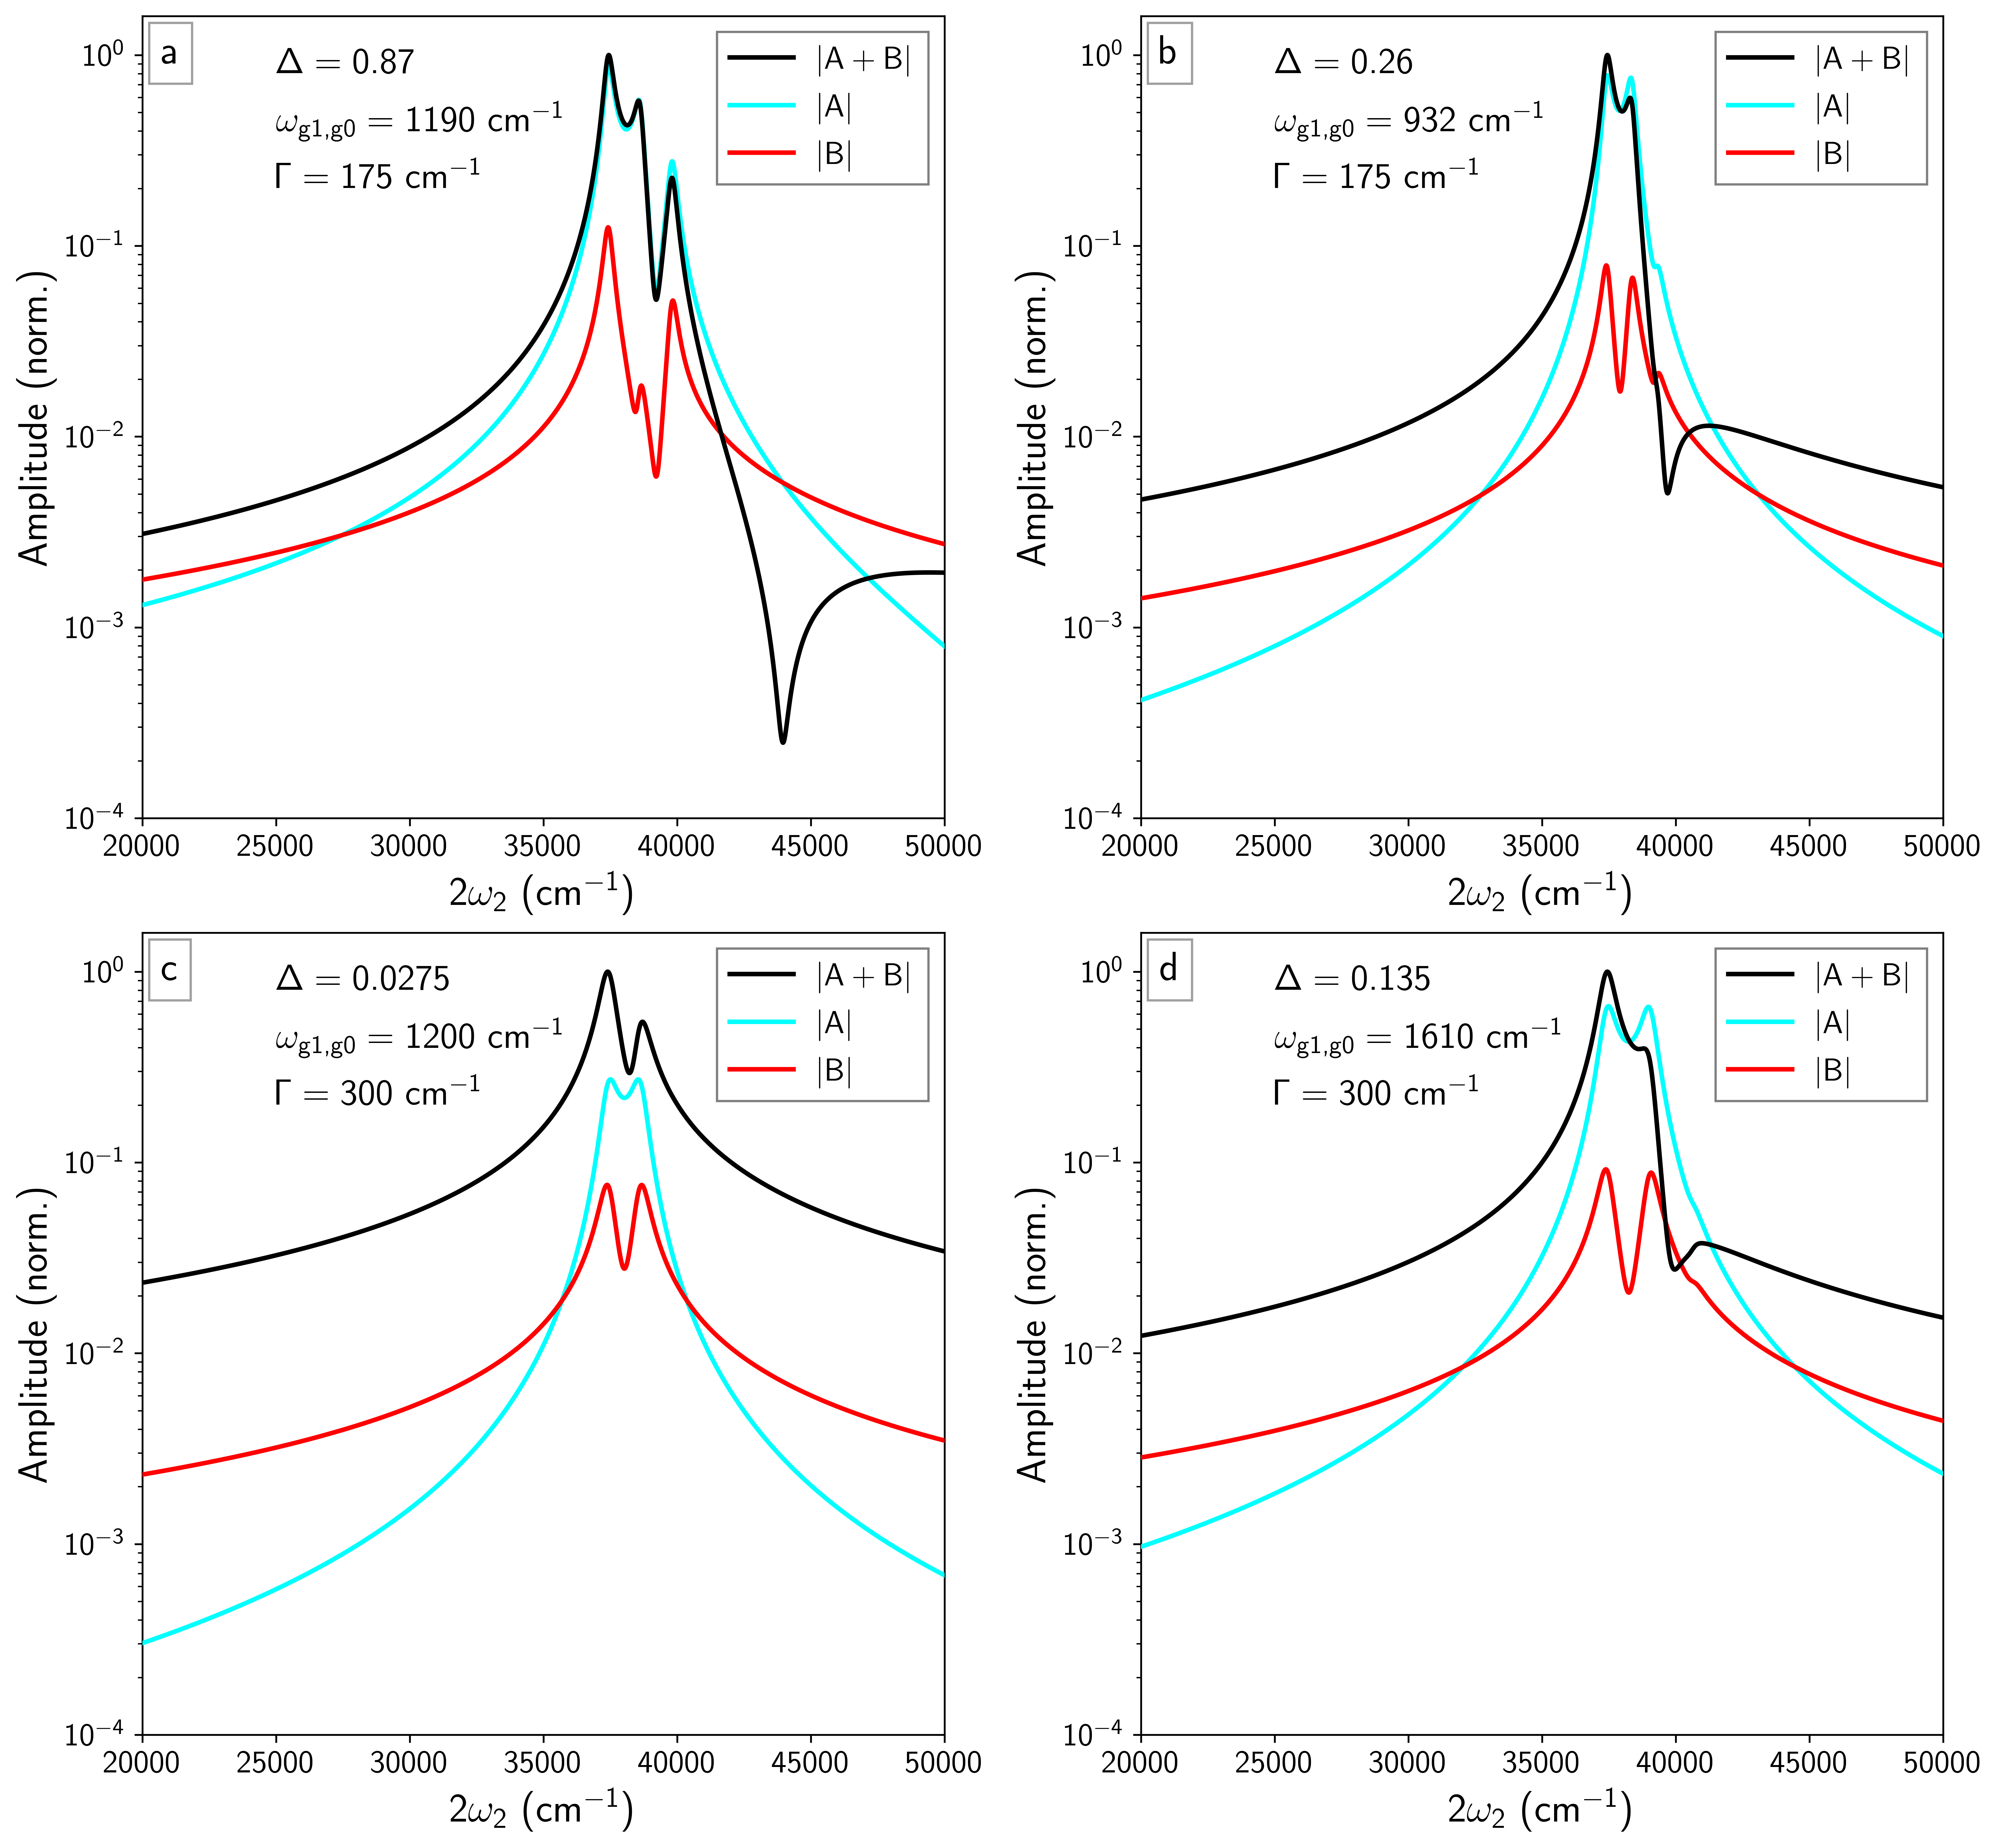
\includegraphics[width=6.675in]{figures/changedelta.png}
	\caption{The impact of offset, vibrational resonance, and linewidth on HDFG spectra. Parameters for (a,b) follow from Myers et al.,\cite{Myers1982} whereas parameters for (c,d) follow from Brennan et al.\cite{Brennan2024}
	In (a-d), the relationship $\max \left(\abs{B}/\abs{A}\right) \sim$ 0.1 at $\Delta = 0.5$ is enforced.
} 
	\label{fig:chgdelta}
\end{figure}

In addition to the linewidth and offset impacting the shape of the HDFG response, the sign of the molecular parameters $M^{ge}_0, \Lambda^{ge}_0, \frac{\partial M^{ge}}{\partial Q} , \frac{\partial \Lambda^{ge}}{\partial Q}$ will significantly impact the HDFG spectrum.
Changing the sign of these parameters can change the sign of $A, B$ and alter the interference between the terms.  
As a specific example (\autoref{fig:chgsign}), we demonstrate the resultant HDFG spectrum for \begin{eqnarray}
	M^{ge}(q) = -1 + 0.04 q,  \\
	\Lambda^{ge}(q) = 0.1 + 0.004 q,
\end{eqnarray}
i.e., $M^{ge}_0 < 0$, $\Lambda^{ge}_0, \frac{\partial M^{ge}}{\partial Q} , \frac{\partial \Lambda^{ge}}{\partial Q} > 0$, keeping $\Delta = 0.5$.
Compared to Figure 3 of the main text, the contributions from the $A, B_1$ and $B_2$ terms to $\Re(\gamma)$ and $\Im(\gamma)$ significantly change.
In particular, $\Re(\gamma)$ and $\Im(\gamma)$ are of similar value in the post-resonance region, eliminating the destructive interference seen in Figure 3 of the main text.
Similar effects have been recently observed in 1D and 2D coherent resonant Raman experiments.\cite{Fumero2020, Batignani2022}
When the sign of $\Delta$, $M(q)$ and $\Lambda(q)$ match, interference in the output lineshape can be observed.
Changing the absolute sign of these parameters can manipulate the interference (\autoref{fig:chgsign2}).
HDFG therefore has the ability to discern the absolute sign of $\Delta$ and assign offsets in potential energy wells for some systems.

%\newpage
\begin{figure}[!htbp]
	\centering
	\includegraphics[width=6.675in]{figures/drsive_chgsign.png}
	\caption{Contributions of $A, B$ to HDFG spectrum for the simple two harmonic well system described by \autoref{Hamiltonian}, except $M^{ge}(q) = -1 + 0.04 q$.
		(a) Potential energy surfaces for a two-well system, (b) 1D HDFG spectrum for $\Delta = 0.5$, $\omega_1 = \omega_{g1, g0}$, (c, d) real and imaginary parts of terms plotted in (b), respectively.
		The spectra are scaled to $\max{(A+B)}$. 
} 
	\label{fig:chgsign}
\end{figure}

\begin{figure}[!htbp]
	\centering
	\includegraphics[width=6.675in]{figures/changedeltaM.png}
	\caption{HDFG spectra for the system described by \autoref{Hamiltonian} with $M^{ge}(q) = M^{ge}_0 + 0.04 q,\ \Lambda^{ge}(q) = 0.01 + 0.004 q$. 
	The respective $\Delta, M^{0}_{ge}$ values are listed above the panels.
	Black trace: $\abs{A+B}$, blue trace: $\abs{A}$, orange trace: $\abs{B}$.
	The spectra are scaled to $\max{\abs{A+B}}$. 
	} 
	\label{fig:chgsign2}
\end{figure}
\newpage
\section{Evaluating the Impact of Static Inhomogeneity on HDFG Spectra}
In this section, the integral
\begin{equation}\label{generalcontour}
	\begin{split}
		\gamma_{ijkl} &= \int_{-\infty}^\infty \mathrm{d}\xi P(\xi) \gamma_{ijkl}(\xi)\\
		&= \frac{\sigma}{\pi}\int_{-\infty}^\infty \mathrm{d}\xi \frac{1}{\sigma^2 + \xi^2} \frac{\eta_{ijkl}}{\left(\Delta_{ga} - \xi\right)\left(\Delta_{ba}+ c\xi\right)} \\
		&= \frac{\eta_{ijkl} \sigma}{\pi} \int_{-\infty}^\infty \mathrm{d}\xi\frac{1}{(\xi + i\sigma)(\xi - i\sigma)} \frac{1}{\Delta_{ga} - \xi} \frac{1}{\Delta_{ba} + c\xi}\\
	\end{split}
\end{equation}
is evaluated for $c=-1$ (electronic state and vibrational state energy fluctuations are anti-correlated) and $c=1$ (electronic state and vibrational state energy fluctuations are correlated).

Integrals such as \autoref{generalcontour} can be evaluated by using the Residue theorem.\cite{MorseFeshbach}
For clarity, we briefly outline the technique.\footnote{See \S 4.5 of Morse and Feshbach \cite{MorseFeshbach} for more details.} 
Consider the integral
\begin{equation}\label{eq:integral}
	\int_{-\infty}^{\infty} \mathrm{d}x f(x).
\end{equation}
Assume \autoref{eq:integral} converges.
If $f(z)$ is analytic on the upper half of the complex plane (except for poles not on the real axis), where $z$ is a complex variable, and $\abs{f(z)}$ asymptotically approaches zero with the form $\abs{Az}^{-m}$, $m > 1$, as $\abs{z} \rightarrow \infty$, then
\begin{subequations}\label{eq:generalcontour}
	\begin{equation}
		\int_{-\infty}^{\infty}  \mathrm{d}x f(x) = 2\pi i \sum_k \Res[f(z_k)],
	\end{equation}
where $\Res[f(z_k)]$ refers to the residue of $f(z)$ at the pole $z_k$ and the sum is taken over all the poles of $f(z)$ in the upper half of the complex plane.\cite{MorseFeshbach}
Note that the residue of an n$^{\text{th}}$ order pole at $z = z_k$ is evaluated as
	\begin{equation}
		\Res[f(z_k)] = \lim_{z \rightarrow z_k} \frac{1}{\left(n-1\right)!} \frac{\mathrm{d}^{n-1}}{\mathrm{d}z^{n-1}} \left[f(z) (z-z_k)^n \right].
	\end{equation}
For first order poles (the cases considered below), $n=1$, so that 
	\begin{equation}
		\int_{-\infty}^{\infty} \mathrm{d}x f(x) = 2\pi i \sum_k \lim_{z \rightarrow z_k} f(z) (z-z_k).
	\end{equation}
\end{subequations}
Note that in \autoref{eq:generalcontour}, the integrals are evaluated along a counter-clockwise contour that wraps all the poles in the positive half of the complex plane. 

\subsection{Anti-correlated Modes}
For anti-correlated modes ($c = -1$), the poles are situated in the complex plane as shown in \autoref{fig:contours}a.
For c = -1, there are four poles: $\pm i \sigma, \Delta_{ga}, \Delta_{ba}$. 
The contour that envelops the upper half of the complex plane has only one pole, $i \sigma$.
Using the residue theorem for a first order pole,\cite{Carlson1990line} we see
\begin{widetext}
	\begin{equation}
		\begin{split}
			\int_{-\infty}^\infty \mathrm{d}\xi P(\xi) \gamma_{ijkl}(\xi) &= 2\pi i \sum_k \lim_{z \rightarrow z_k} P(z) \gamma_{ijkl}(z) (z - z_k)\\
			&= 2\pi i \frac{\eta_{ijkl} \sigma}{\pi} \lim_{z \rightarrow i\sigma} \frac{1}{(z + i\sigma)(z- i\sigma)} \frac{1}{\Delta_{ga} - z} \frac{1}{\Delta_{ba} - z} (z - i \sigma)\\
			&= 2 \eta_{ijkl} \sigma i \lim_{z \rightarrow i\sigma} \frac{1}{z + i\sigma} \frac{1}{\Delta_{ga} - z} \frac{1}{\Delta_{ba} - z}\\
			&= 2\eta_{ijkl} \sigma i \frac{1}{2i\sigma} \frac{1}{\Delta_{ga} - i\sigma} \frac{1}{\Delta_{ba} - i\sigma}\\
			&= \frac{\eta_{ijkl}}{\left(\Delta_{ga}-i\sigma\right)\left(\Delta_{ba}-i \sigma\right)}.\\
		\end{split}
	\end{equation}
\end{widetext}


\subsection{Correlated Modes}
For correlated modes ($c = 1$), the poles are situated in the complex plane as shown in \autoref{fig:contours}b.
We evaluate along the contour that encloses the poles $\{i\sigma, -\Delta_{ba}\}$.
Since $i\sigma \neq -\Delta_{ba}$, i.e., the poles are nondegenerate, we have two first order poles, giving
\begin{widetext}
	\begin{equation}
		\begin{split}
			\int_{-\infty}^\infty \mathrm{d}\xi P(\xi) \gamma_{ijkl}(\xi) &= 2\pi i \sum_k \lim_{z \rightarrow z_k} P(z) \gamma_{ijkl}(z) (z - z_k)\\
			&= 2\pi i \frac{\eta_{ijkl} \sigma}{\pi}  \lim_{z \rightarrow i\sigma} \frac{1}{(z + i\sigma)(z - i\sigma)} \frac{1}{\Delta_{ga} - z} \frac{1}{\Delta_{ba} + z} \left(z - i \sigma\right) \\ 
			&+ 2\pi i \frac{\eta_{ijkl} \sigma}{\pi} \lim_{z \rightarrow -\Delta_{ba}} \frac{1}{(z + i\sigma)(z - i\sigma)} \frac{1}{\Delta_{ga} - z} \frac{1}{\Delta_{ba} + z} \left(z + \Delta_{ba}\right)\\
			&= 2 \eta_{ijkl} i \sigma \left(\frac{1}{2 i \sigma} \frac{1}{\Delta_{ga} - i\sigma} \frac{1}{\Delta_{ba} + i\sigma} \right) + 2\eta_{ijkl} i \sigma \left(\frac{1}{\sigma^2 + \Delta_{ba} ^2} \frac{1}{\Delta_{ga} + \Delta_{ba}} \right)\\
			&= \frac{\eta_{ijkl}}{\Delta_{ba} + i \sigma} \left(\frac{1}{\Delta_{ga} - i \sigma} + \frac{2i\sigma}{(\Delta_{ba} - i \sigma)(\Delta_{ga} + \Delta_{ba})}\right).\\
		\end{split}
	\end{equation}
\end{widetext}


\begin{figure}[!htbp]
	\centering
	\includegraphics[width=6.675in]{figures/contour.png}
	\caption{Poles (blue dots) and contours (black lines) used to evaluate \autoref{generalcontour} for (a) anti-correlated ($c=-1$) and (b) correlated ($c=1$) modes. 
	The contours are oriented counter-clockwise.
	} 
	\label{fig:contours}
\end{figure}

\section{References}
% Create the reference section using BibTeX:
\bibliography{library.bib}

\end{document}
%


